% !TEX root = ../patchEmbeddings_review.tex

\section{Introduction}\label{sec:intro}

\emph{Instance segmentation} is a task of computer vision consisting in assigning each pixel of an image to an object instance. %, where the number of instances is usually not known in advance. 
% The most success in instance segmentation (IS) has been achieved by applying deep learning. %\cite{he2017mask,romera2016recurrent,liu2018affinity}. 
There are two main types of successful deep learning approaches to instance segmentation: proposal-based and proposal-free methods. 
Proposal-based methods consist of two steps: object detection, for example by finding bounding boxes, and assigning pixels to the detected objects. These approaches have proven to be highly successful in instance segmentation competitions like MS COCO \cite{lin2014microsoft} and CityScapes \cite{cordts2016cityscapes}. 
On the other hand, proposal-free methods adopt a bottom-up approach by directly grouping pixels into instances. Recently, there has been a growing interest for such methods that do not involve object detection, since, in certain types of images like the ones we focus on in this work, object instances cannot be approximated by bounding boxes and are usually larger than the field of view of the model.  

 
% A graph partitioning algorithm is used to obtain object instances.
Some recent successful proposal-free approaches \cite{januszewski2018high,meirovitch2016multi,liu2016multi} tackle instance segmentation by predicting, for a given patch of the input image, whether or not each pixel in the patch is part of the same instance associated to the central/anchor pixel. 
These masks are then repeatedly predicted, in a sliding window style, across the entire image and 
the final object-instances are obtained by aggregating predictions from overlapping masks.
In the following, we will refer to these patch predictions as \emph{\maskname masks}.

In this work, we propose a novel proposal-free segmentation method that is also based on the prediction of \maskname masks. However, our approach comes with the following four main advantages.
Firstly, our model concurrently predicts all \maskname masks, one for each pixel, by using a fully-convolutional approach and comes then with a much lower computational cost compared to previous patch-based methods iteratively predicting one instance at the time, one mask after the other \cite{januszewski2018high,meirovitch2016multi}.
Secondly, our approach predicts \maskname masks in a low dimensional latent representation, which allows great memory savings and let us apply the method to large volumetric images of neuron tissue \cite{arganda2015crowdsourcing}. 
Thirdly, the proposed approach aggregates predictions from overlapping \maskname masks without the need of any extra parameter or threshold;
and, finally, all final object-instances are obtained concurrently, as opposed to previous methods predicting them one-by-one with subsequent conflict resolution. 
% by extracting a set of affinities that are then used as signed weights of a graph representing the image, so that each node corresponds to a pixel

% Despite the recent successful application of patch-based methods, so far no study has been conducted to compare them with 

We also carry out a systematic study to compare the proposed model with another really common proposal-free method that has been recently successfully applied both to natural \cite{liu2018affinity,Gao_2019_ICCV} and biological \cite{lee2017superhuman,wolf2018mutex,bailoni2019generalized} images. This alternative method is sketched in Fig. \ref{fig:main_figure}a and consists of a fully-convolutional network predicting, for each pixel, a small set of short- and long-range affinities, i.e. neighborhood relations representing how likely it is for a pair of pixels to belong to the same object instance. 
\TODO{} Our comparison on neuron segmentation shows how... (equally efficient, results, etc...)


% In this work, we focus on a proposal-free method, where a Convolutional Neural Network (CNN) is trained to predict, for every pixel $i$ in the image, a patch of fixed size representing a probability mask of the instance object to which pixel $i$ belongs. The mask predicted in each patch is centered at the corresponding pixel $i$ and represents then a dense local neighborhood structure of pixel $i$. Whenever the object instance associated to pixel $i$ is bigger than the size of the patch, only a partial probability mask of the object is predicted. 
% In the following, we will call these masks as \patch or LSPM.

% [A naive way to predict one $K\times K$ \patch  for each pixel in an image would be to use a fully convolutional model with $K^2$ output channels, where each channel represents a pixel of the corresponding mask. However, this approach would not scale up well with increasing sizes $K$.]

% Our first contribution is a fully convolutional model that predicts, for every pixel $i$, a representation of the associated $i$-th self-probability mask in a lower dimensional space (see Fig. \ref{fig:main_figure}). This is possible due to the fact that, among all possible neighborhood structures represented by local self-probability masks, only few of them are associated to occurring ground truth binary masks. Thus, the information included in the predicted self-probability masks can be easily encoded in a lower dimensional latent space. 



% As a second contribution, we propose two methods for converting the predicted per-pixel self-probability masks into edge weights of a graph representing the image, so that each node corresponds to a pixel and a graph clustering algorithm is used to obtain the final instance segmentation... \TODO{Parameter-free alg. to compute edge weights; experiments; summary of sections}
% One of the two methods results in a pipeline that is as efficient as the currently winning method of the CREMI challenge \emph{(more efficient actually, because of LMC...), but achieves better accuracies and, as our results shows, outputs more consistent neighborhood structures...}.
% The second proposed method yields a parameter-free algorithm achieving competitive performances, yada yada yada... 


\begin{figure}[t]
\centering
        % \includegraphics[width=0.4\textwidth,trim=0.25in 0.25in 0.68in 0.36in,clip]{./figs/SSBM_experiments.pdf} % 0.45
        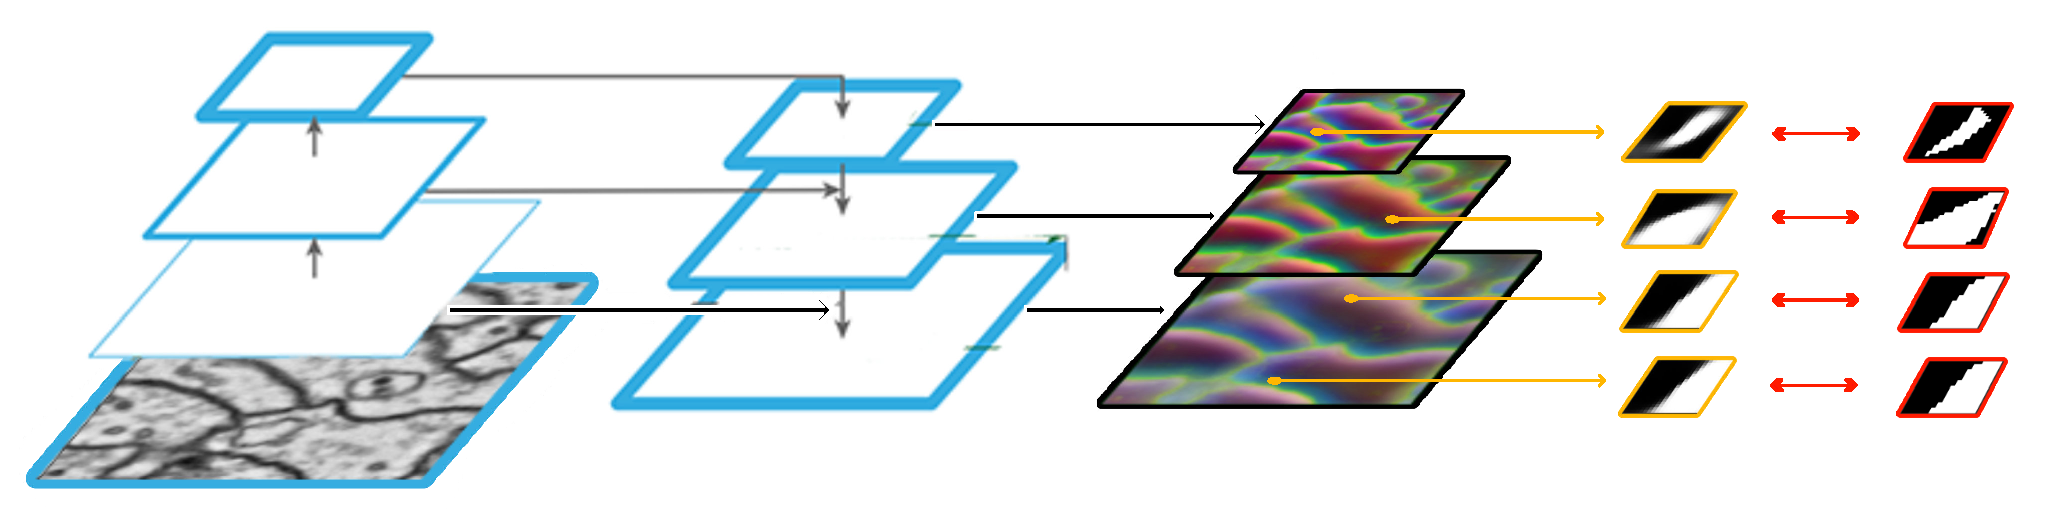
\includegraphics[width=\textwidth]{./figs/main_image.pdf} % 0.45
        \caption{A.) Predicting a sparse stencil of short- and long-range affinities. b) Predicting all patches (that it was actually the main proposal of PatchPerPix)...}
    \label{fig:main_figure}
\end{figure}


